%!TEX root = ./template-skripsi.tex

\subsection{Sprint 2 Report}
Berikut merupakan report dari sprint ke-2 yang dilakukan pada tanggal 1 juni -7 juni 2022.

\begin{table}[H]
	\caption{\textit{Sprint-2 backlog}}
	\label{sprint2_backlog}
	\begin{tabular}{@{} |p{0.5cm}|p{5cm}|p{5cm}|p{2cm}| @{}}
		\hline
		\textbf{No} & \textbf{\textit{Story}} & \textbf{\textit{Task}} & \textbf{\textit{Status}} \\
		\hline
		1 & \multirow{3}{5cm}{Create, Read, Updte, dan Delete untuk Pencatatan Pemberian pakan} & Membuat view pakan bulanan & Completed\\
		\cline{1-1}\cline{3-4}
		2 & & Membuat view pakan harian & Completed\\
		\cline{1-1}\cline{3-4}
		\hline
	\end{tabular}
\end{table}

\begin{enumerate}[1.]
\item View pakan bulanan
\begin{figure}[H]
	\centering
	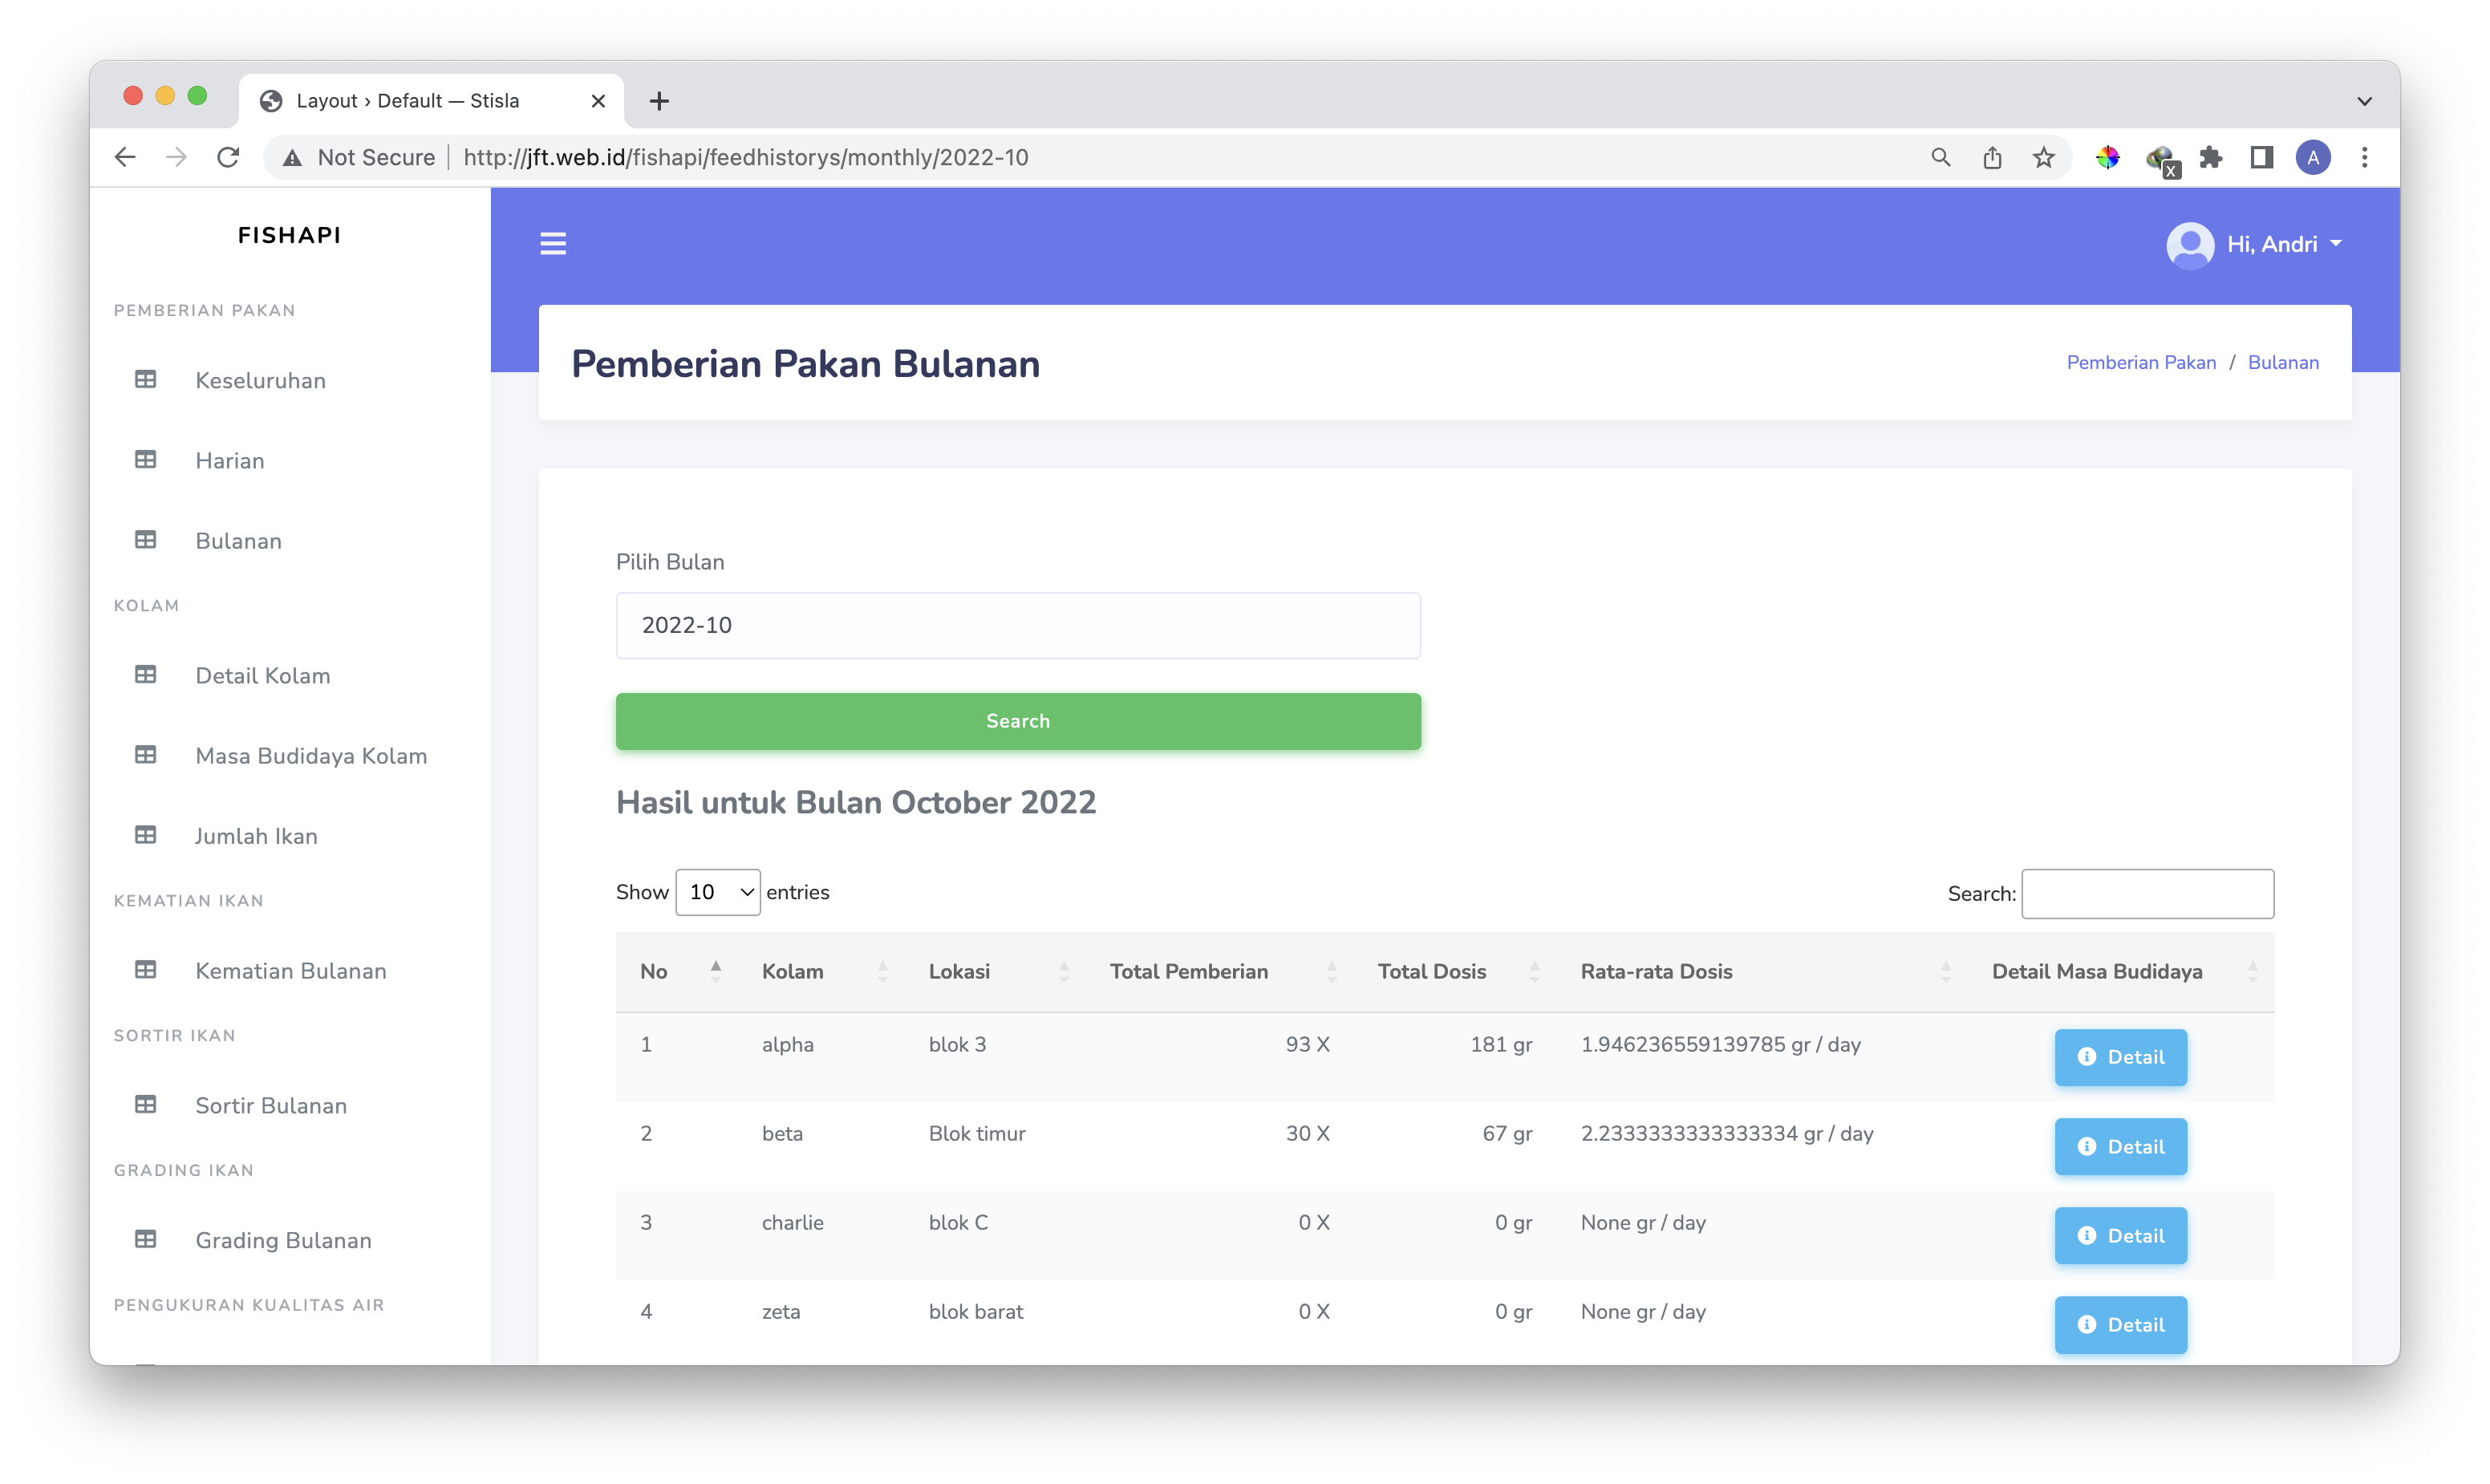
\includegraphics[width=1\textwidth]{gambar/Sprint02/view_pakan_bulanan}
	\caption{View pakan bulanan}
	\label{fig:view_pakan_bulanan}
\end{figure}
	
\item View pakan harian
\begin{figure}[H]
	\centering
	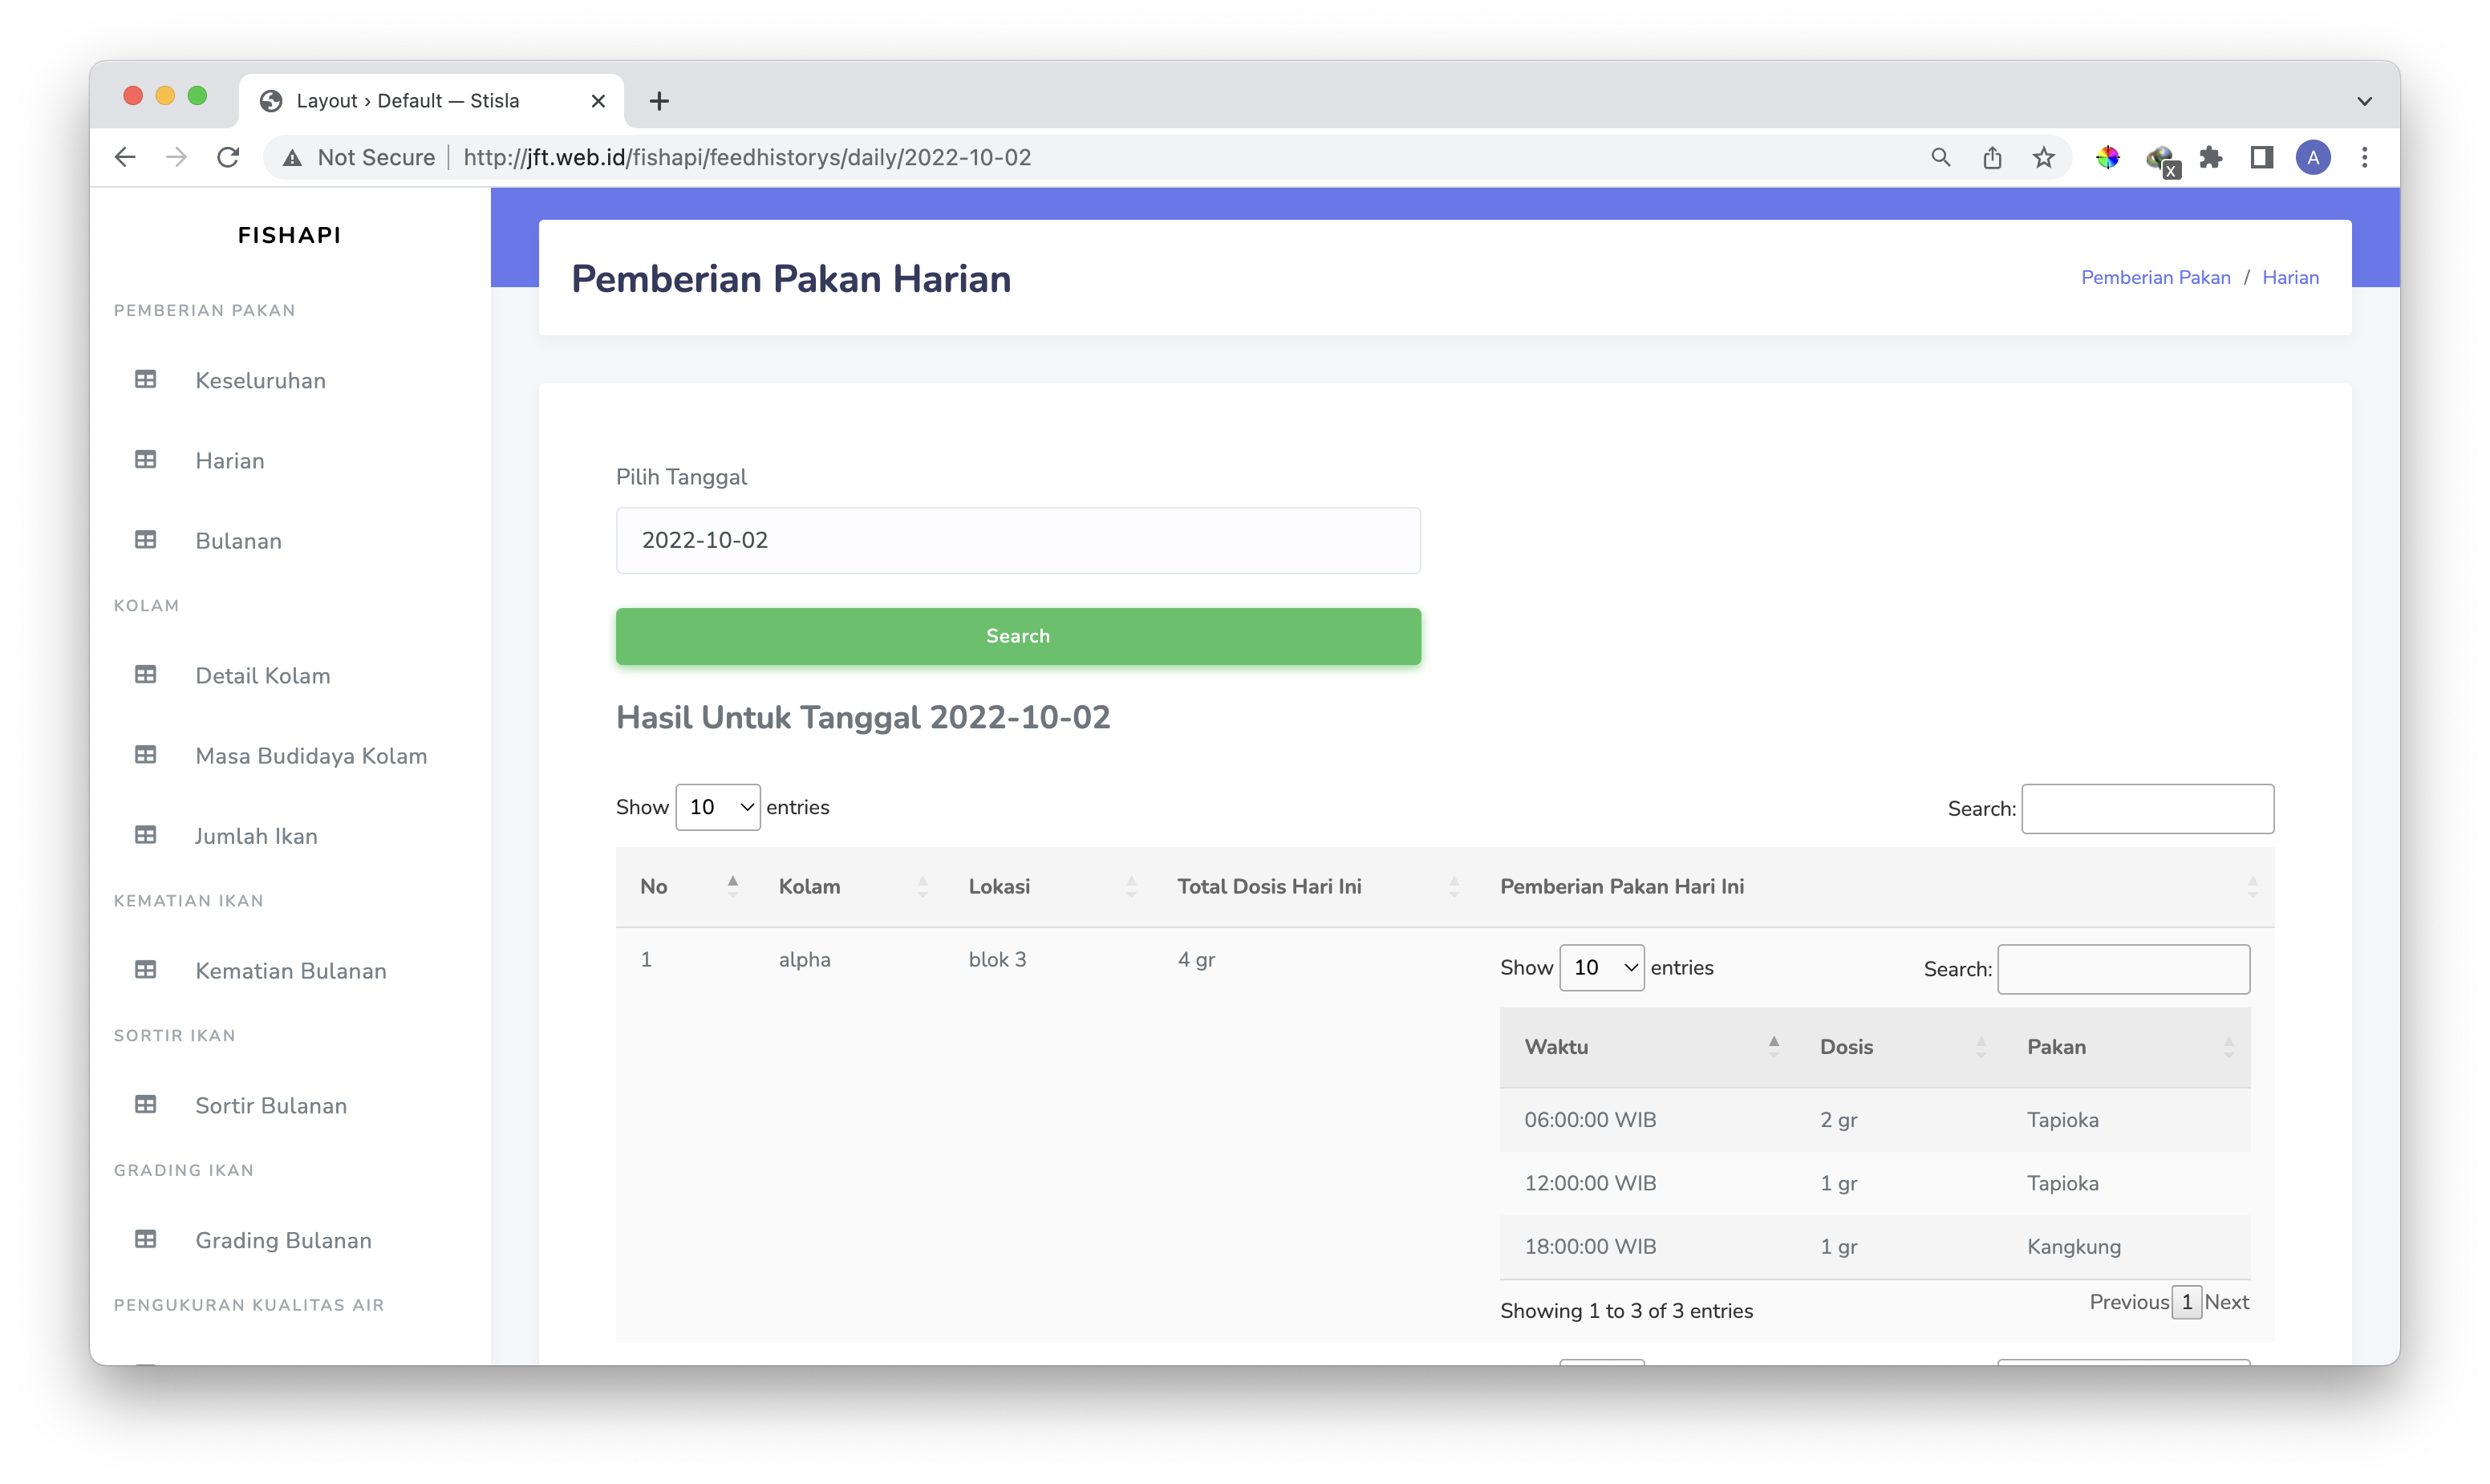
\includegraphics[width=1\textwidth]{gambar/Sprint02/view_pakan_harian}
	\caption{View pakan harian}
	\label{fig:view_pakan_harian}
\end{figure}
\end{enumerate}